\chapter{Specifications} \label{specifications}

\section{Functional Description}\label{functional-description}

The Roa Logic APB4 GPIO is a configurable, fully parameterized soft IP to
enable general connectivity to a APB4 based Master (Host) It is fully
compliant with the \emph{AMBA APB v2.0} bus protocols.

The IP contains a single Master Interface to connect to the APB4 Host
and a user defined number of General Purpose IO, configurable as a
bi-directional bus as shown below:

\begin{figure}[tbh]
	\centering
	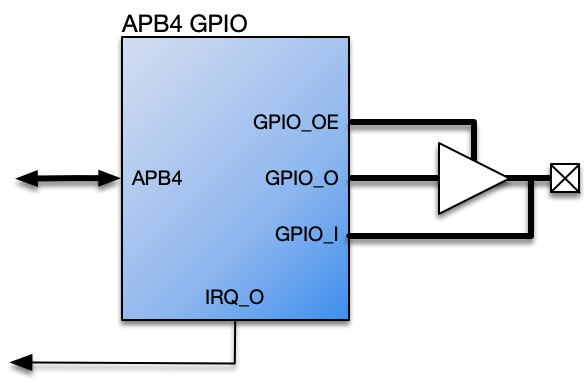
\includegraphics{assets/img/apb4-gpio-sys.png}
	\caption{Bidirectional IO Pad}
	\label{fig:apb4-gpio-sys}
\end{figure}

The core operates synchronously with the APB4 Bus Clock. The core synchronises all inputs to the APB4 Bus Clock domain.

\section{Operating Modes}\label{operating-modes}

The core supports bidirectional IO pads as shown in Figure 3, where each
IO can be programmed to operate in push-pull or open-drain mode. The mode of each IO is
defined via the MODE register.

\begin{longtable}[]{@{}|p{2cm}p{12cm}@{}}
	\textbf{Note:} & \\
	\endhead
	 & IO Pads are not implemented within the APB4 GPIO core --
	this technology specific capability is the responsibility of the
	designer.\\
\end{longtable}

\subsection{Push-Pull Mode}\label{push-pull-mode}

In push-pull mode, the \texttt{GPIO\_O} bus is driven from an internal \texttt{OUTPUT}
register and \texttt{GPIO\_OE} is controlled via the
DIRECTION register

Logically the push-pull mode is configured as follows:

\begin{figure}[tbh]
	\centering
	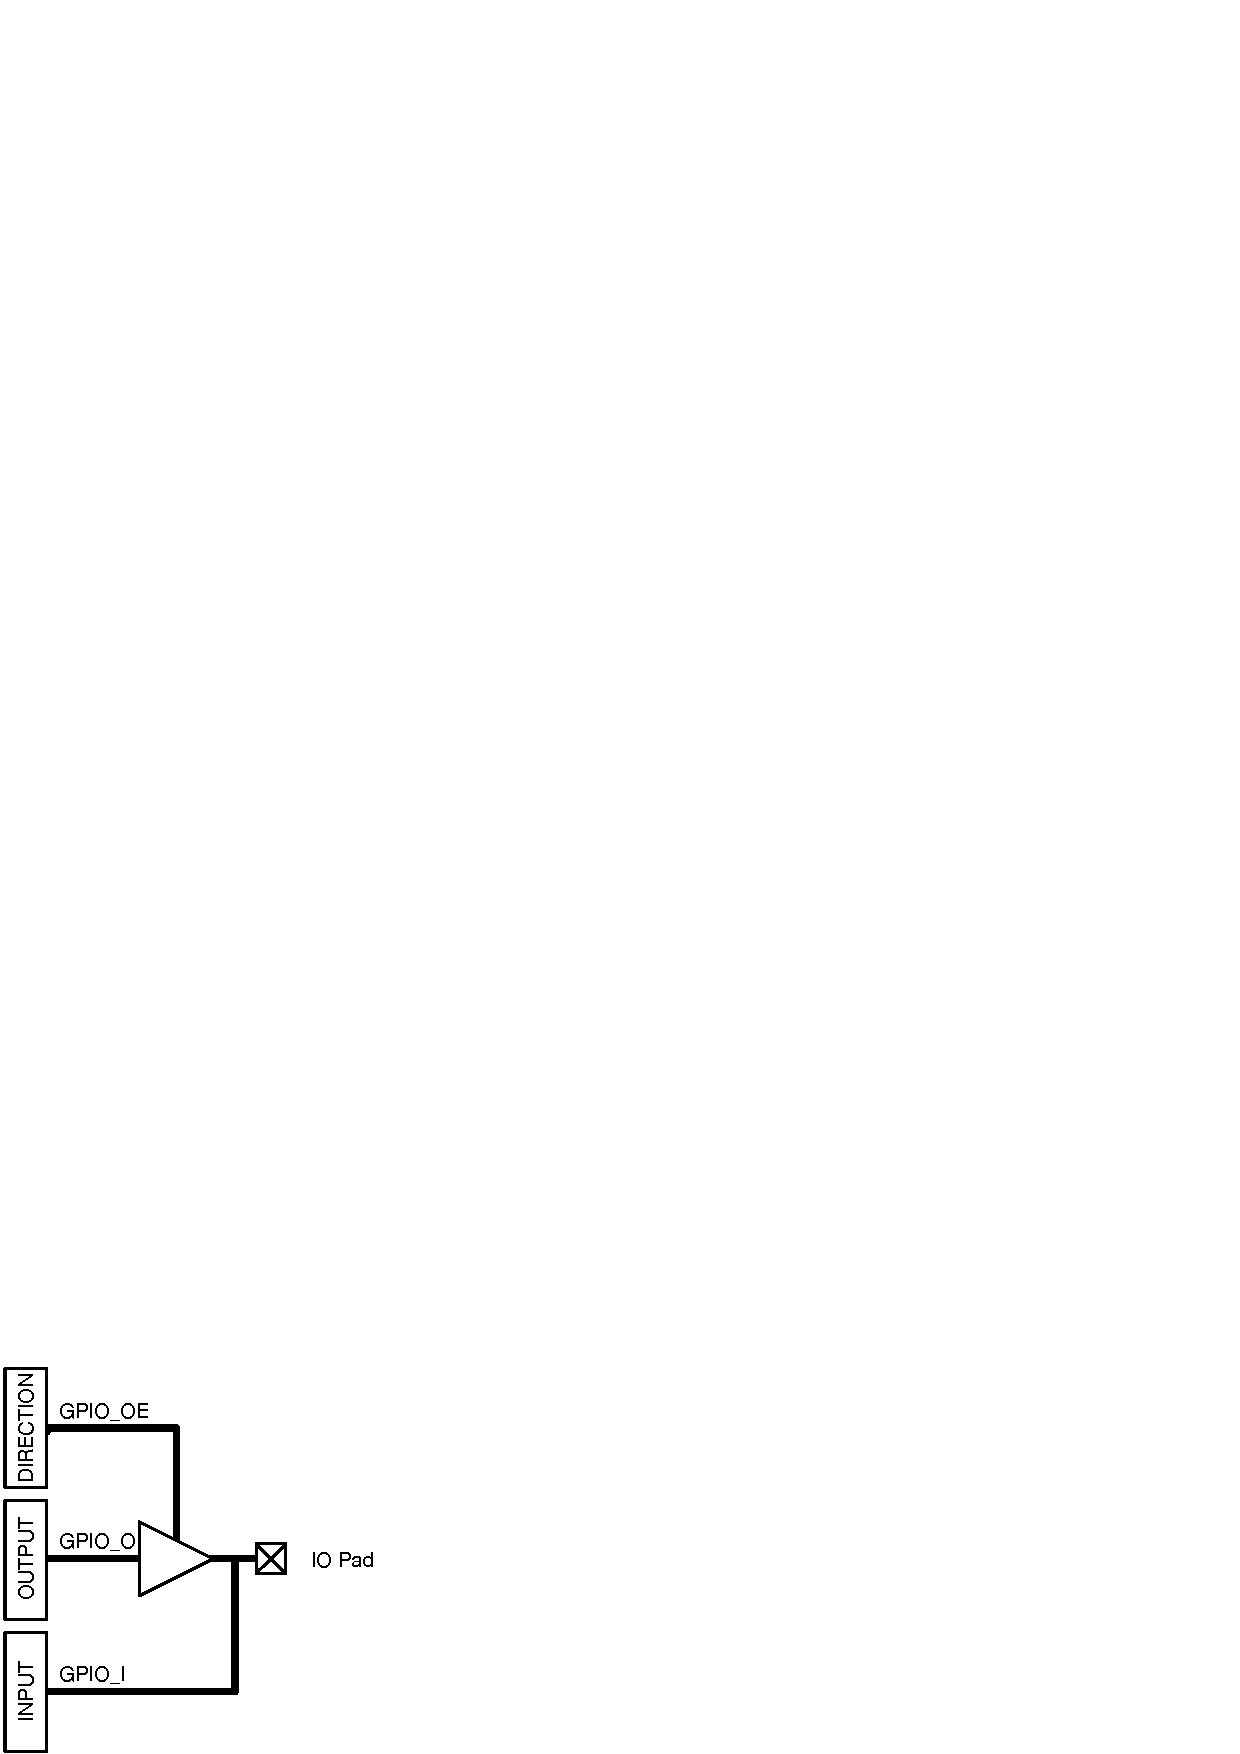
\includegraphics{assets/img/apb4-gpio-pp.png}
	\caption{Push-Pull Configuration}
	\label{fig:apb4-gpio-pp}
\end{figure}


\subsection{Open-Drain Mode}\label{open-drain-mode}

In open-drain mode, GPIO\_O is always driven low (`0') and individual
GPIO\_OE signals set to enable (i.e. Logic `0') or high-Z (Logic `1') at
the output buffer corresponding to the value of the OUTPUT register.

\begin{figure}[tbh]
	\centering
	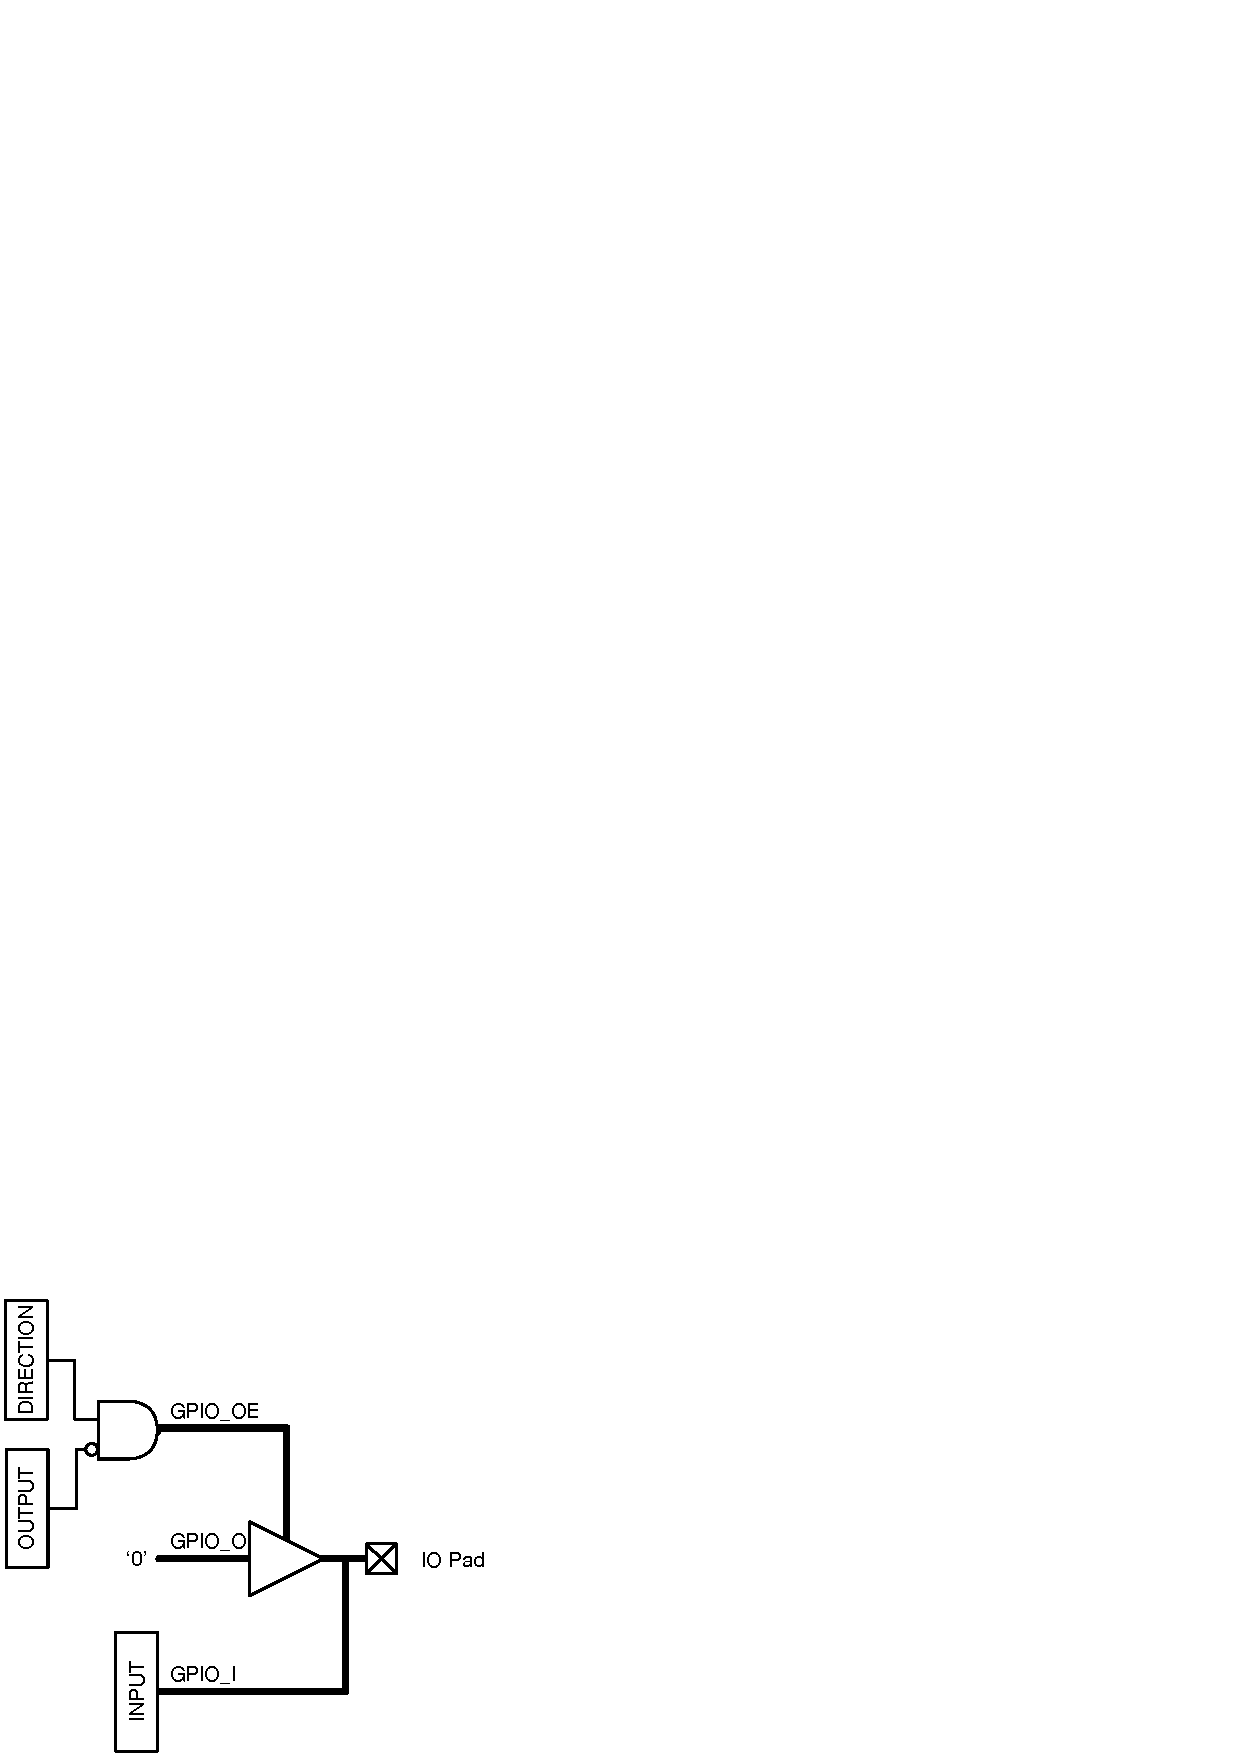
\includegraphics{assets/img/apb4-gpio-od.png}
	\caption{Open Drain Configuration}
	\label{fig:apb4-gpio-od}
\end{figure}

\subsection{Pad Inference}\label{pad-inference}

The inclusion of technology specific IO Pads is not part of the APB4
GPIO core and instead left to the designer. Pads may be behaviourally
inferred however as follows:

\texttt{PAD[n] = GPIO\_OE[n] ? GPIO\_O[n] : 1'bz;}

\texttt{GPIO\_I[n] = PAD[n];}
